% !TeX spellcheck = en_US
\documentclass[./main.tex]{subfiles}
\begin{document}


\let\texteuro\euro
\subsection{Monezitation Strategy}
The monetization strategy of Commed is mainly based on a percentage of the value of the commercial agreement contracts. When a contract has been finally set, an invoice will be generated. The value of the invoices depends on the value of the generated contract in order to make the invoices affordable for all types and sizes of companies. Therefore, in the first four years, the search of the companies and the other features will be free. After these beginning years, it is something to study and plan if some other features can become freemium.
\\
\\
In order to get more publications in the first few years and popularize our service quickly, the first three publications will be free for any company. The next ones will cost 250 € per year, which will not depend on the size of the company publishers.
In addition, any kind of publication could get a better position in the search by paying monthly. The fee of this kind of advertising will be up to 450 € per month and the position will depend on how much the company pays for that advertising.
\\
\\
Therefore, there are three possible incomes:
\begin{itemize}
	\item 5\% commission of each contract generated.
	\item Publish a 4\supindex{th}, 5\supindex{th},..., n\supindex{th} offer cost 250 € per new offer each year. \\Publishers have 3 free publications.
	\item Payments for advertising by month, the payment will be chosen by the customer in the same way it is done on instagram and facebook. The more the company pays for the advertising, the more the offer will appear. The maximum fee should be 450 € per month.
\end{itemize}
As the search will be free, the companies could be able to negotiate and set the contract out of our reach. In order to sort this inconvenience out, Commed will finally generate the contract making this process so easy and the invoice very affordable as the payment is only the 5\% of the contract.
\subsection{Marketing Strategy}
According to the marketing strategy, it has been set that the main focus in the first years will be getting the small and medium sized companies, in order to quickly popularize the platform and create small business ecosystems. For example, the main ecosystems to focus on in the first year will be in order of importance:
\begin{itemize}
	\item Restauration, butchers and other food providers.
	\item Food industry and supermarkets.
	\item Organizations for seasonal work to get temporary contracts.
	\item Cleaning services.
	\item Security services.
	\item Logistic services.
\end{itemize}
After creating the small ecosystem, the focus will be on strengthening the ecosystem and widening the smaller ones in order to join with the others and make them become a greater one.

Explain why door-to-door strategy

Costs : 
Advertising on Linkedin because we are a B2B business
Freelance Salesman


\subsection{Speculation and flow chart}
In order to create the simulation of the revenue, a speculation has been done on how many contracts will be held by our application in a month. This conjecture has been simulated over the first four years of the company. The revenue functions consists on these three variables:
\begin{itemize}
	\item The income from the percentage of the contract between the entities. This variable has the main weight of the function as it is the main income generator. Mean value for small business contracts : 1000€. Mean value for big business contracts : 4000€. 
	\item The revenue from the paid publications. In order to ease the simulation and know how many publications will be paid, a relaxation of the problem has been made. The paid publications ratio has been calculated with an approximation, which also is directly correlated with the amount of contracts held.
	\item The income from the payments for advertising a publication. This variable has also been approximated making a correlation from the number of contracts.
\end{itemize}
According to the costs, its function depends on these variables:
\begin{itemize}
	\item The cost of paying developers, which can be splitted into junior or senior developers.
	\item Marketing cost.
	\item As the platform will be growing, the costs of the server will be higher. Despite that, it is thought about creating a serverless backend using AWS Lambda to minimize this cost and only pay for the requests.
\end{itemize}
Three scenarios have been made in order to show a possible but different projection of the incomes generated by the platform:
\begin{itemize}
	\item A pessimistic scenario, where the number of contracts increases in a linear way amongst the four years.
	\item An optimistic scenario, in which the contracts’ function has an exponential form.
	\item A more realistic scenario, which also has linear function in the first years but in the lasts, it gets more the way of an exponential function.
\end{itemize}
\subsection{Pessimistic Scenario}
Number of contracts at the end of each year : 
\begin{table}[]
\begin{tabular}{|l|l|l|l|l|}
\hline
\textbf{Year}                     & 1  & 2   & 3   & 3   \\ \hline
\textbf{Small Business Contracts} & 65 & 100 & 170 & 280 \\ \hline
\textbf{Big Business Contracts}   & 0  & 0   & 40  & 73  \\ \hline
\end{tabular}
\end{table}
\begin{table}[H]
	\centering
	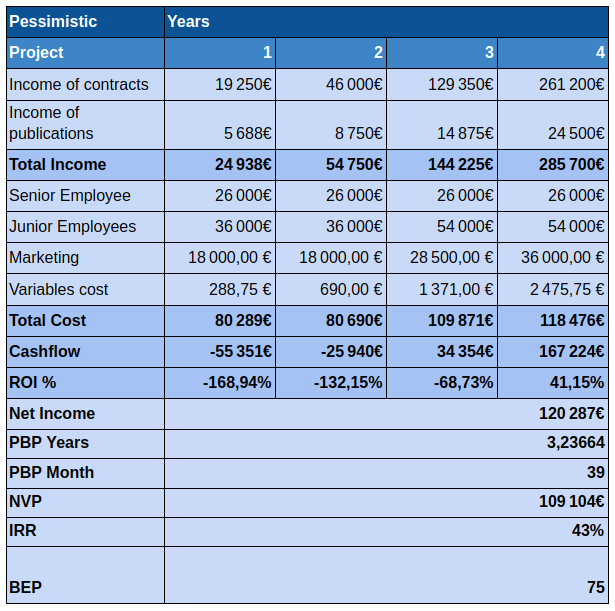
\includegraphics[width=11.3cm]{pessimistic.png}
	\caption{Pessimistic Cash Flow}
	\label{tab:pessimistic}
\end{table}

\subsection{Realistic Scenario}
Number of contracts at the end of each year : 
\begin{table}[]
\begin{tabular}{|l|l|l|l|l|}
\hline
\textbf{Year}                     & 1  & 2   & 3   & 3   \\ \hline
\textbf{Small Business Contracts} & 77 & 160 & 230 & 412 \\ \hline
\textbf{Big Business Contracts}   & 0  & 0   & 60  & 137 \\ \hline
\end{tabular}
\end{table}
\begin{table}[H]
	\centering
	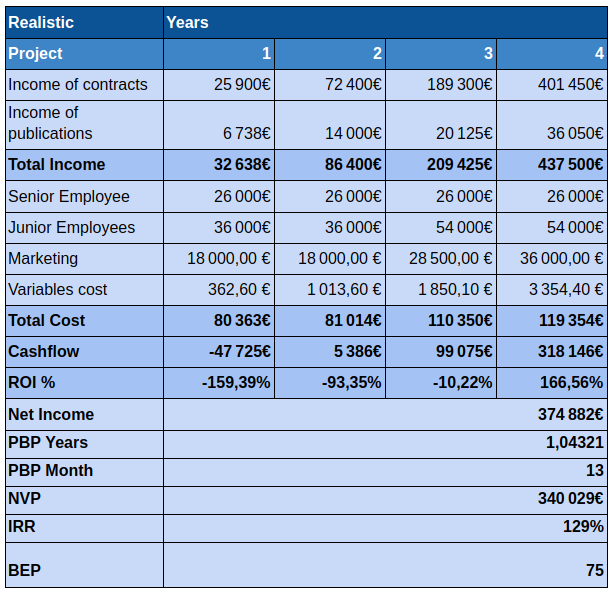
\includegraphics[width=11.3cm]{realistic.png}
	\caption{Realistic Cash Flow}
	\label{tab:realistic}
\end{table}

\subsection{Optimistic Scenario}
Number of contracts at the end of each year : 
\begin{table}[]
\begin{tabular}{|l|l|l|l|l|}
\hline
\textbf{Year}                     & 1  & 2   & 3   & 3   \\ \hline
\textbf{Small Business Contracts} & 85 & 200 & 270 & 500 \\ \hline
\textbf{Big Business Contracts}   & 0  & 0   & 74  & 180 \\ \hline
\end{tabular}
\end{table}
\begin{table}[H]
	\centering
	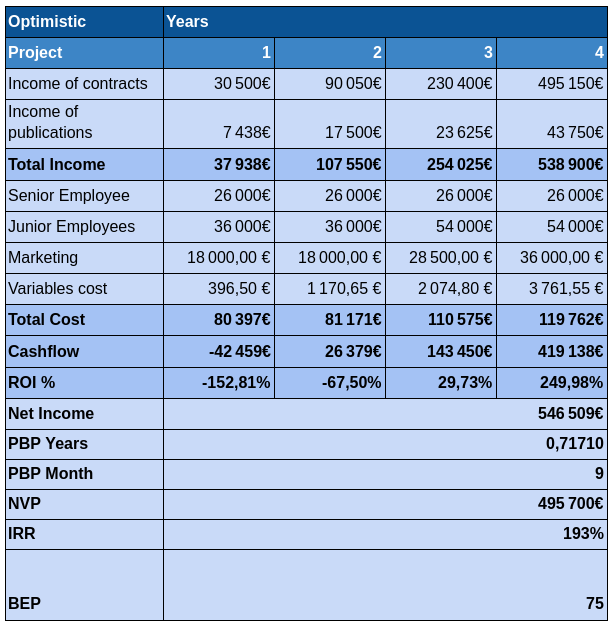
\includegraphics[width=11.3cm]{optimistic.png}
	\caption{Optimistic Cash Flow}
	\label{tab:optimistic}
\end{table}

\subsection{Economic indices comparison between scenarios}
All information related to the simulation and prediction about the first four years of the platform can be found in the spreadsheet attached to this document. Even though, the cash flows of each scenario can be found in \textit{Tables \ref{tab:pessimistic}, \ref{tab:realistic} and \ref{tab:optimistic}.}
In this section, we will begin by comparing the three scenarios using the different indexes calculated above. \\
\\
First, we want to show you the \texttt{ROI} index between the different scenarios, which can be found in Table \ref{tab:roi}. The \texttt{ROI} has been calculated every year, as it is more significant to us to analyze this information. Although it can be found that the \texttt{ROI} index in the first year is similary between the scenarios, the pessimistic scenario has some challenges to increase the ROI so as to be positive while optimistic and, actually, the realistic appear to have a better return on investment.
\begin{table}[H]
	\centering
	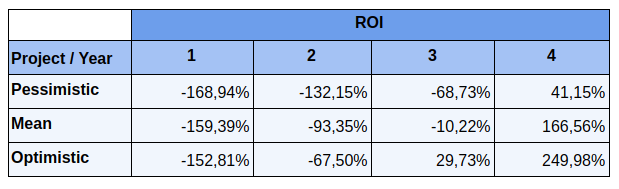
\includegraphics[width=11cm]{roi.png}
	\caption{ROI Index comparison between the three scenarios}
	\label{tab:roi}
\end{table}
According to the other indices, mostly all of them have better values in the optimistic scenario. One of the most valuable indices is the \texttt{PBP} in terms of months. Here, we can see that the optimistic has only 9 months of \texttt{PayBack Period}. On the other hand, realistic scenario is a promising case, as in only one year and a month we would be able to recover the cost of the investment.
\\
\\
Although \texttt{ROI} gave us bad values, specially in the pessimistic scenario, we can see that in all the scenarios the \texttt{IRR} is positive. That gave us good information to know if someone is going to invest on the company. The only one index that has the same behaviour in all the cases it is the \texttt{BEP}, which is calculated monthly. That is because the costs are fixed, as the lifecycle of the software would be large.
\begin{table}[H]
	\centering
	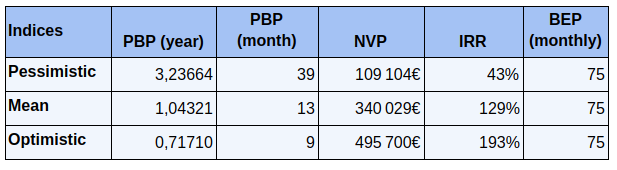
\includegraphics[width=11cm]{indices.png}
	\caption{Indices comparison between the three scenarios}
	\label{tab:indicies}
\end{table}

In Figure \ref{fig:cashflow}, we can see the contracts’ function of all the scenarios and the total cost function, which is the same in all scenarios. In the optimistic scenario, we will start to recover the initial investment at the beginning of the first year whereas in the worst case, we will start generating benefits at the beginning of the third year.
\begin{figure}[h]
	\centering
	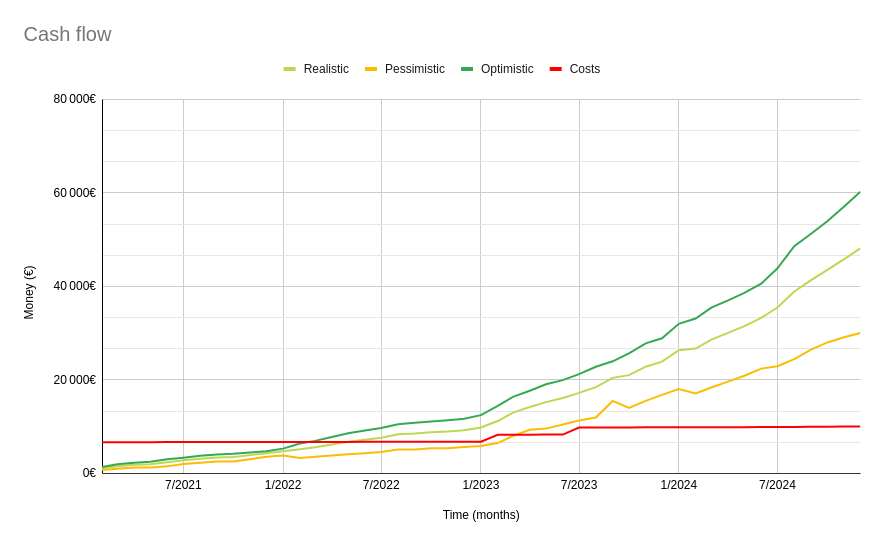
\includegraphics[width=15cm]{CashFlow.png}
	\caption{Cash flow of the different revenue function from scenarios and cost function}
	\label{fig:cashflow}
\end{figure}

\end{document}
